\documentclass{article}
\usepackage{amsmath}
\usepackage{amssymb}
\usepackage{tikz}
\usepackage{cancel}
\usetikzlibrary{arrows.meta, positioning}
\tikzset{%
    block/.style = {draw=black,rectangle,thick,
        minimum height=2em, text width=20em, align=center},
    line/.style = {draw=cyan, line width=3pt, 
        -{Triangle[length=6pt, width=8pt]}, shorten >=2pt, shorten <=2pt},
}


\begin{document}
\newcommand{\norm}[1]{\left\Vert#1\right\Vert}
{\large Continuum mechanics}
\vskip 0.2in
\noindent
In a flow problem on a 2D domain {\Large $\Omega$}, the primary physical variable is the velocity field $\text{\Large $u : \Omega \rightarrow \mathbb{R}^2$}$.
This field evolves in accord with continuum versions of Newton's laws of motion.
The Cauchy momentum equation is the {\large $F = ma$} of continuum mechanics. It can be stated as an integral conservation law quantified
over all pieces of space, $\Omega_0 \subset $ {\Large $\Omega$}:
\begin{align*}
\frac{d}{dt} \int_{\Omega_0(t)} \rho u(\hat{x}) \,d\hat{x} &= \int_{\Omega_0}F(\hat{x})\,d\hat{x} + \oint_{\partial \Omega_0} \sigma(\hat{x})\cdot\hat{n}\,d\hat{x}.\\
\end{align*}
This says that the rate of change of total momentum (pointwise $\rho u$) in the piece $\Omega_0$, as it moves with the material,
is accounted for by body forces (pointwise $F$) and the \textit{tractions} (pointwise $\sigma\cdot\hat{n}$ on the boundary of the piece of space),
which measure internal forces due to the interaction of nearby material elements. $\sigma$, a $2\times 2$ matrix for each point in $\Omega$, is the \textit{Cauchy stress tensor}, and its specification
depends on the material being modelled. Conservation of mass is written as
\begin{align*}
\frac{d}{dt} \int_{\Omega_0(t)} \rho(\hat{x})\,d\hat{x} = 0,
\end{align*}
which says that the a small piece $\Omega_0$, as it moves with the material, has constant total mass.


\newpage
\vskip 0.2in
{\large The Navier-Stokes equations}
\vskip 0.2in
\noindent
The incompressible Navier-Stokes equations are a Cauchy momentum equation ($F = ma$),
along with a stronger version of mass conservation called incompressibility (conservation of volume):
    $$\oint_{\partial\Omega_0}u(\hat{x})\cdot\hat{n}\,d\hat{x} = 0 \text{\quad\quad for all pieces $\Omega_0 \subset \Omega$}.$$
These equations model an incompressible Newtonian fluid
with traction forces $\sigma\cdot\hat{n}$ being decomposable into two parts:
\begin{itemize}
    \item A viscous force (which causes adjacent particles
in the fluid to tend to the same speed, like a ``momentum diffusion''),
    \item and an isotropic force which pushes
    small pieces of the material apart from each other, in order for the flow to obey the incompressibility constraint.
\end{itemize}
This second force is due to the pressure field
$\text{\Large $p : \Omega \rightarrow \mathbb{R}$}$,
which is a Lagrange multiplier
for the constraint. The Navier-Stokes equations, in integral ``primal-dual'' form, to be solved for both
$u$ and the Lagrange multiplier $p$, are
\begin{equation}\label{navier_stokes}
\begin{split}
    \frac{d}{dt} \int_{\Omega_0(t)} \rho u(\hat{x}) \,d\hat{x} &=
        \int_{\Omega_0}F(\hat{x})\,d\hat{x} + \oint_{\partial \Omega_0} \mu\nabla u(\hat{x})\cdot \hat{n}\,d\hat{x}
            -\oint_{\partial\Omega_0} p(\hat{x})\hat{n}\,dx\\
    \text{and\quad} \oint_{\partial\Omega_0}u(\hat{x})\cdot\hat{n}\,d\hat{x} &= 0 \text{\quad\quad for all pieces $\Omega_0 \subset \Omega$}.
\end{split}
\end{equation}
$\text{\huge $\mu$}$ is the dynamic viscosity, which controls the momentum diffusion force.

\newpage
\vskip 0.2in
{\large Steady flow and the steady Stokes equations}
\vskip 0.2in
A steady flow is one for which the velocity $u$ does not change with time. This means that
a particle moving through the fluid will always follow the same path.
The left-hand side of the Navier-Stokes equations \eqref{navier_stokes} describes the change of momentum in the piece $\Omega_0$ as it moves
with the material. The \textit{Reynolds transport theorem} rephrases this as a change of momentum internal to the piece $\Omega_0$,
if it were to stay still, and the total momentum that the piece loses or gains at the boundary as it flows: \eqref{navier_stokes}
is rewritten as
\begin{equation*}
\cancel{\int_{\Omega_0} \rho \frac{\partial u(\hat{x})}{\partial t}\,d\hat{x}}
+ \oint_{\partial \Omega_0}\rho u(u\cdot \hat{n})\,d\hat{x}
      = \int_{\Omega_0}F(\hat{x})\,d\hat{x} + \oint_{\partial \Omega_0} \mu\nabla u(\hat{x})\cdot \hat{n}\,d\hat{x}
            -\oint_{\partial\Omega_0} p\hat{n}\,dx\\
\end{equation*}
for which the time-dependent component is set to zero, resulting in the steady Navier-Stokes equations. There is still a non-linear term on
the left-hand side, describing the advection (the fluid is still moving, even though it is steady):
$$
\text{\Large Non-linear!}\longrightarrow
\oint_{\partial\Omega_0}\rho u(u\cdot \hat{n})\,d\hat{x} \longleftarrow \text{\Large Non-linear!}
$$
If this term is ignored, the resulting equations are linear and model a steady-state flow for which there is a well-defined velocity,
but the material doesn't ``actually move'' --- this turns out to be a useful approximation if the \textit{Reynolds number} is small:
    {\large $$Re = \frac{\rho \norm{u} L}{\mu} \ll 1 \quad\Longrightarrow\quad \text{momentum diffusion} \gg \text{momentum advection}.$$}
The result is the steady Stokes equations:
\begin{equation}\label{steady_stokes}
\begin{split}
        -\oint_{\partial \Omega_0} \mu\nabla u(\hat{x})\cdot \hat{n}\,d\hat{x}
            &= \int_{\Omega_0}F(\hat{x})\,d\hat{x}
            -\oint_{\partial\Omega_0} p(\hat{x})\hat{n}\,dx\\
    \text{and\quad} \oint_{\partial\Omega_0}u(\hat{x})\cdot\hat{n}\,d\hat{x} &= 0 \text{\quad\quad for all pieces $\Omega_0 \subset \Omega$}.
\end{split}
\end{equation}

\newpage
\vskip 0.2in
{\large The finite element method for flow problems: A network of pieces of space}
\vskip 0.2in
Continuum mechanics provides the foundation for understanding of fluid motion, and the Navier-Stokes equations
are the primary model for the prediction of fluid behaviour in engineering.
The domain and initial/boundary conditions can be arbitrarily complex. For example, fluid motion is often simulated
through a digital surface model of a real-world object or system created in computer-aided design software.
On the other side of the coin, fluid models are very often used in modern film, both live action and animated,
and all relevant geometry can be adjusted by artists for a desired visual effect.

In applications, the Navier-Stokes equations are primarily
solved on a computer, and a computer works with both finite data and finite precision.
Galerkin methods 
are particularly amenable to computer implementation, so much so that the whole process of geometric modelling, boundary condition handling,
residual minimisation, and solution reconstruction, can be automated. The finite volume method and finite element method are

\newpage
\vskip 0.2in
{\large Solving the Stokes equations numerically}
\vskip 0.2in
\noindent
The solution {\large $(u,p)$} has infinite degrees of freedom.
The conservation laws are quantified over arbitrary pieces of the domain,
giving an infinite number of equations, as integrals equated to $0$. These residuals can be thought of
as ``trials'', testing if a supposed solution satisfies the conservation laws.
Why not choose finite degrees of freedom for approximate {\large $(\tilde{u}, \tilde{p})$},
and the same number of trial equations to go with them?
Suppose $\tilde{u} \in \Phi^u$ and $\tilde{p} \in \Phi^p$, where
    $$\Phi^u = \text{span}\left\{\phi^u_1,\cdots,\phi^u_{2n_u}\right\},\quad 
        \Phi^p = \text{span}\left\{\phi^p_1,\cdots,\phi^p_{n_p}\right\}$$
are, respectively, spaces of vector velocity fields and of scalar pressure fields, both compatible with the integral equations.

% A finite number of pieces $\Omega^{u}_1,\cdots,\Omega^u_{n_u}$, which might tessellate the interior of $\Omega$, can be chosen.
% If the residual for the linearized momentum equation is zero for all of these, this means ``momentum is approximately conserved''.
% Another finite number of pieces $\Omega^{p}_1,\cdots,\Omega^p_{n_p}$ could also be chosen to check that ``$\tilde{u}$ is approximately
% incompressible''. This is called a finite volume method, and is a good idea for conservation laws such as Poisson's equation)
% but a pure FVM, as just described, turns out not to lead to a stable method for the Stokes equations.
A finite number of pieces $\Omega_0$ could be chosen.
If the residual for the linearized momentum equation is zero for all of these,
and the residual for the incompressibility constraint is zero, this can be taken to mean ``momentum is approximately conserved'',
and ``$\tilde{u}$ is approximately non-compressing''.
This is called a finite volume method, and is a good idea for conservation laws such as Poisson's equation.
A pure FVM, as just described, turns out not to lead to a stable method for the Stokes equations.

In an attempt to find an alternative finite set of equations, the Stokes equations can be written in the \textit{weak form}
\begin{equation}\label{steady_stokes_weak_form}
\begin{split}
        \int_{\Omega} \mu\nabla u(\hat{x})\cdot \nabla\psi^u(\hat{x})\,d\hat{x}
            &= \int_{\Omega}F(\hat{x})\psi^u\,d\hat{x}
            +\int_{\Omega} p(\hat{x})\nabla\cdot\psi^u\,dx \text{\quad for all $\psi^u \in \Psi^u$}\\
    \text{and\quad} -\int_{\Omega}u(\hat{x})\cdot\nabla\psi^p\,d\hat{x} &= 0 \text{\quad for all $\psi^p \in \Psi^p$}.
\end{split}
\end{equation}
Although maybe less clear than the original form, this is a sort of ``rearrangement'' of the infinite system of equations given in terms of fluxes
(analagous to a rebasis of a linear system).
For the continuous PDE, the ``trial spaces'' $\Psi^u$ and $\Psi^p$ are certain generalised function spaces.
For example, for the discretized method, why not choose $\Psi^u = \Phi^u$ and $\Psi^p = \Phi^p$?


\newpage
\vskip 0.2in
{\large The Taylor-Hood mixed finite element method}
\vskip 0.2in
The Stokes flow problem at the top of this poster is a Dirichlet boundary value problem, with a no-slip condition ($u = (0,0)$) on the top
and bottom walls, and unit-speed in-flow and out-flow $u = (-1,0)$ at the left and right boundaries. This approximates the effect of motion
($\dot{x} = 1$)
of the obstruction through an infinite cylinder, as long as the boundaries are far enough away.

This problem has been solved with a \textit{finite element method}, effectively by choosing some discrete function spaces, plugging in approximations to the weak
form of the Stokes equations, then rearranging everything into a large, sparse linear system.
In a finite element method,
``test spaces'' $\Phi^\cdot$ and ``trial spaces'' $\Psi^\cdot$ are constructed as the spans of basis functions built on a domain tessellation
(such as a triangulating mesh).
These basis functions are zero except on a small number of triangles localised around some point on the mesh, a property which leads to
sparsity of the resulting matrix and right-hand side.

Let the $\Psi$ spaces be equal to the $\Phi$ spaces (called a ``Bubnov--Galerkin method'').
The velocity space $\Phi^u$, for simplicity, can be a product space of scalar function spaces: $\Phi^u = \Phi^{u,s} \times \Phi^{u,s}$,
with basis functions
    $$\Phi^u = \text{span}\left\{\phi^u_{1x},\phi^u_{1y},\cdots,\phi^u_{n_ux},\phi^u_{n_uy}\right\}.$$

The boundary values can be accounted for by letting $\tilde{u}_\Gamma$ be some arbitrary approximating function which satisfies the boundary condition,
and restricting $\Phi^u$ to be zero on the boundary. The resulting linear system is
\begin{equation}
\begin{split}
    \sum_{i=1}^{n_u}\left[
        u_{ix}\int_\Omega\mu\nabla\phi_{ix}^u:\nabla\psi_j^u\,d\hat{x}
        +
        u_{iy}\int_\Omega\mu\nabla\phi_{iy}^u:\nabla\psi_j^u\,d\hat{x}
    \right]
    +
    \sum_{i=1}^{n_p} p_i\int_\Omega \phi_i^p\nabla\cdot\psi^u_j\,d\hat{x}
    =
    \int_\Omega\nabla\tilde{u}_\Gamma:\nabla\psi_j^u\,d\hat{x},\\
    \text{\quad $j=1,\cdots,n_u$}.
\end{split}
\end{equation}







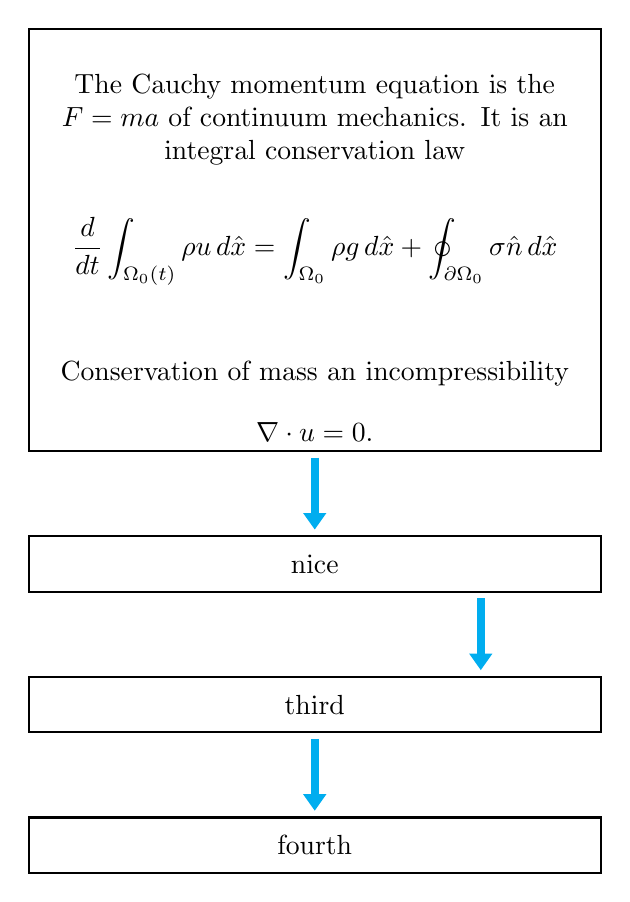
\begin{tikzpicture}[node distance = 2cm, auto] 
    \node [block] (init) {
\begin{center}
The Cauchy momentum equation is the $F = ma$ of continuum mechanics. It is an integral conservation law
\end{center}
\begin{align*}
\frac{d}{dt} \int_{\Omega_0(t)} \rho u \,d\hat{x} &= \int_{\Omega_0}\rho g\,d\hat{x} + \oint_{\partial \Omega_0} \sigma\hat{n}\,d\hat{x}\\
\end{align*}
\begin{center}
Conservation of mass an incompressibility
\begin{align*}
\nabla\cdot u = 0.
\end{align*}
\end{center}
}; 
    \node [block, below=30pt of init] (expert) {
nice}; 
    \path [line] (init) -- (expert); 
    \node [block, below=30pt of expert] (third) {third}; 
    \path [line] ([xshift=6em]expert.south) -- ([xshift=6em]third.north); 
    \node [block, below=30pt of third] (fourth) {fourth}; 
    \path [line] (third.south) -- (fourth.north); 
\end{tikzpicture}

\end{document}

